While iterating through design decisions the idea was to make the GUI as familiar as possible. In many dialogues
and popular graphical user interfaces a similar layout is encountered - menubar on top, left to right and
top to bottom reading, bottom right buttons for completing the task see figure \ref{fig:guiex}. Because
of its purpose and the way its used the GUI looks more as a dialogue window - simple window that helps 
generate a file/configuration and its used for a short amount of time.

\begin{figure}[htp]
\centering
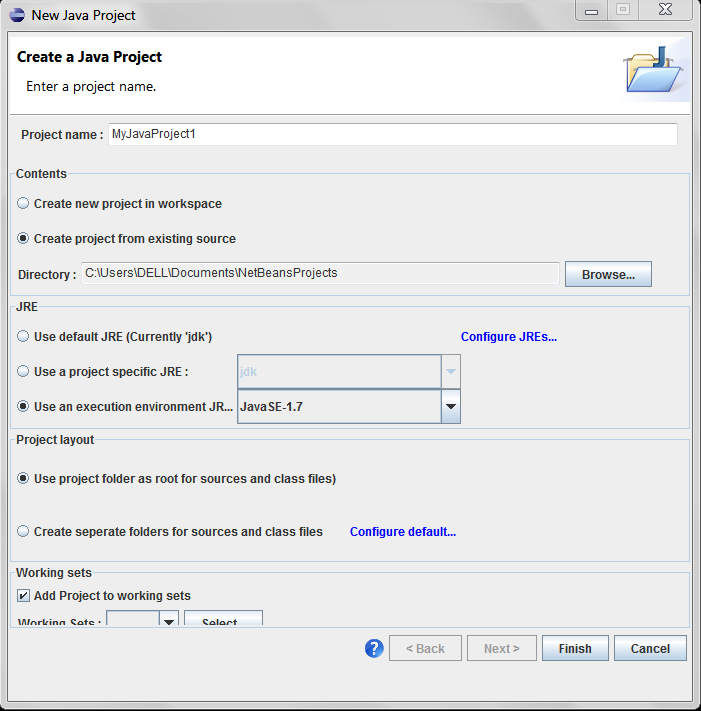
\includegraphics[scale=0.6]{Figures/gui_example1.png}
\caption{Example of a dialogue used for configuration of projects used in Eclipse editor}
\label{fig:guiex}
\end{figure}

The most important parameters - target IP address and client IP address,
are located at the top left corner of the window. Other parameters text fields are located from left  to right top to bottom
based on their relevance. That's why bottom left is located the button for generating the XML configuration
file hence finishing the process.

\begin{figure}[htp]
\centering
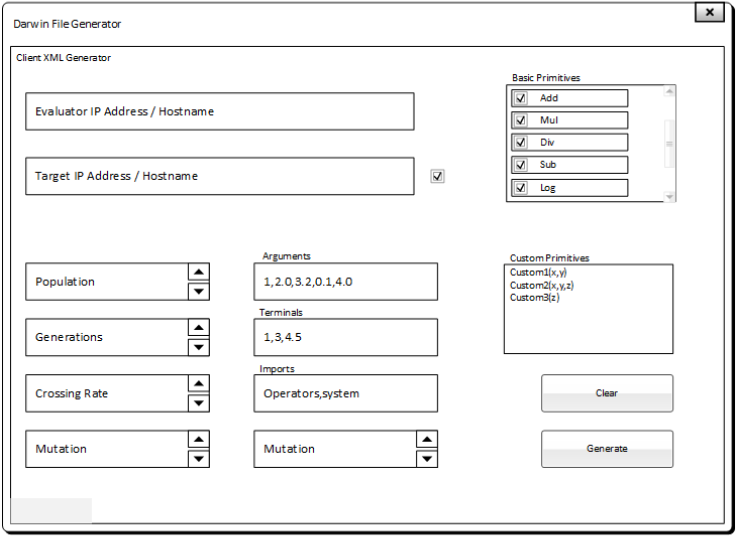
\includegraphics[scale=0.6]{Figures/guiit.png}
\caption{One of the iterations of the GUI showing all the possible parameters}
\label{fig:guiit}
\end{figure}

In the first iteration of the design additional features like adding custom primitives and selecting imports
for those custom primitives were added as you can see in figure \ref{fig:guiit}. However after discussion with the client it was later
decided that these features are part of the more advanced functionality of the framework. It was unnecessary to implement them in the GUI
 since they were available in the code where they would be 
normally reached and modified from a more experienced users that would use this functionality. The final iteration of the GUI design
 looked as displayed in figure \ref{fig:guiit}
 it